%%%%%%%%%%%%%%%%%%%%%%%%%%%%%%%%%%%
\chapter{Redes Complexas}\label{redes-complexas}
%%%%%%%%%%%%%%%%%%%%%%%%%%%%%%%%%%%
% \redcomment{Falar o que são redes, para que serve, os estudos, as metricas... (5 ou 6 paginas)}

Neste capítulo apresentamos uma visão geral dos conceitos, perspectivas e aplicações de redes complexas, 
bem como as principais definições e métricas utilizadas no presente trabalho. 
% Assume-se que o leitor tenha um conhecimento sobre a terminologia utilizada 
% em teoria dos grafos.

%%%%%%%%%%%%%%%%%%%%%%%%%%%%%%%%%%%
\section{Introdução}
%%%%%%%%%%%%%%%%%%%%%%%%%%%%%%%%%%%

O interesse pela forma e complexidade como entidades\footnote{Por entidade entende-se qualquer coisa, concreta ou 
abstrata, que tenha importância em um dado domínio.} estão conectadas na sociedade moderna tem ganhado força na última 
década. Em meio a este interesse existe a ideia das redes que~\cite{Easley2010} definem como um padrão de interconexões 
entre um conjunto de entidades. Essas redes podem aparecer em vários contextos e podem ser vistas sob várias perspectivas.

As redes sociais, de acordo com~\cite{Easley2010}, são compostas por coleções de laços sociais entre amigos e apresentam 
grande crescimento de complexidade ao logo da história humana devido aos avanços tecnológicos que facilitaram o deslocamento 
geográfico, a comunicação global e a interação social. 
% Esta evolução tecnológica enfraqueceu a natureza tradicional das estruturas de tais redes, no entanto, as enriqueceram em outras dimensões.

\cite{Dunbar1992} mostra que indivíduos tendem a se organizar em grupos e que tais indivíduos possuem uma capacidade 
cognitiva de manter relações sociais estáveis com um número limitado de indivíduos (uma variação entre 100 e 230). Mais 
tarde, \cite{Goncalves2011} mostraram que essas características se mantêm em \textit{redes sociais online} (OSNs - \textit{Online Social 
Networks}), mostrando que a complexidade entre as ligações dos indivíduos tendem a manter-se mesmo com a evolução tecnológica.

Podemos identificar sistemas na sociedade atual que possuem estruturas semelhantes às de uma rede, i.e., possuem elementos 
interconectados. Essas estruturas se tornaram tão complexas de modo que uma pequena alteração em um dado ponto pode refletir 
por todo o sistema de forma catastrófica, como sistemas tecnológicos e econômicos, onde pequenas alterações podem causar falhas 
em cascatas ou crises financeiras.

Redes podem ser identificadas em vários outros contextos, como redes de fornecedores em operações de manufatura, \textit{sites} com 
redes de usuários ou redes de \textit{sites} que se interligam através de hiperlinks e empresas de mídia com suas redes de 
anunciantes. Em tais formulações, muitas vezes o foco acaba sendo mais na estrutura da própria rede do que na sua complexidade 
como um todo, onde alterações em elementos centrais podem causar reações inesperadas.

O estudo sobre redes e suas conexões, conhecido também como análise de redes complexas, é um tema interdisciplinar que 
permeia diversas áreas do conhecimento como Ciência da Computação, Matemática, Física, Biologia e Sociologia. De acordo 
com~\cite{Boccaletti2006}, uma rede complexa pode ser formalmente representada como um grafo, uma ferramenta matemática 
originada dos estudos de Euler, que inicialmente a utilizou para formalizar o problema das pontes de Königsberg, 
conhecido também como o problema das sete pontes \citep{Euler1956}.

A análise de redes complexas e a teoria dos grafos são utilizadas em diversas outras áreas, dentre elas a sociometria, 
que utiliza-se desses conceitos para realizar a modelagem dos atores e suas respectivas ligações, sendo os atores 
representados por nodos e suas ligações representadas por arestas. Com a rede social gerada, ou sociograma como é chamada na 
sociometria, é possível identificar: (i) os líderes aceitos, (ii) atores que por algum motivo estão marginalizados, 
(iii) grupos que se fecharam com algum interesse em comum, (iv) atores responsáveis por unir um ou mais 
grupos sem serem membros de tais grupos, também chamados de estrelas, (v) atores pontes, que são responsáveis por unirem um ou 
mais grupos dos quais fazem parte, e por fim, (vi) atores isolados, que não fazem parte de qualquer grupo~\citep{Moreno19531978}.

Com o surgimento e popularização das OSNs, tais estudos se intensificaram devido ao grande número de pessoas
nessas redes e também pelo conteúdo gerado, podendo estes conteúdos serem desde simples mensagens de texto ou até mesmo conteúdo
multimídia, como fotos e vídeos. De acordo com~\cite{Benevenuto2012}, OSNs são ambientes ricos para o estudo de várias áreas 
da Ciência da Computação, incluindo sistemas distribuídos, padrões de tráfego na Internet, mineração de dados, sistemas 
multimídia e interação humano-computador.


% % Durante a última década tem havido uma crescente fascinação do público com a "conexão" complexo da sociedade moderna. No coração deste fascínio é a idéia de uma rede - um padrão de interconexões entre um conjunto de coisas - e encontra-se redes que aparecem em discussão e comentários sobre uma enorme gama de tópicos. A diversidade de contextos em que as redes são chamadas é de fato tão grande que vale a pena adiar definições precisas para um momento enquanto primeiro recontagem alguns dos exemplos mais salientes.
% % Over the past decade there has been a growing public fascination with the complex “connectedness” of modern society. At the heart of this fascination is the idea of a network — a pattern of interconnections among a set of things — and one finds networks appearing in discussion and commentary on an enormous range of topics. The diversity of contexts in which networks are invoked is in fact so vast that it’s worth deferring precise definitions for a moment while we first recount a few of the more salient examples.
% % 
% % Para começar, as redes sociais que habitam-as coleções de laços sociais entre amigos - têm crescido em complexidade ao longo da história humana, devido aos avanços tecnológicos que facilitam viagens distantes, a comunicação global ea interação digital. O último meio século tem visto essas redes sociais partem muito mais radicalmente de suas bases geográficas, um efeito que enfraqueceu a natureza tradicionalmente locais de tais estruturas, mas os enriqueceram em outras dimensões.
% % To begin with, the social networks we inhabit—the collections of social ties among friends — have grown steadily in complexity over the course of human history, due to technological advances facilitating distant travel, global communication, and digital interaction. The past half-century has seen these social networks depart even more radically from their geographic underpinnings, an effect that has weakened the traditionally local nature of such structures but enriched them in other dimensions. 
% % 
% % A informação que consumimos tem uma estrutura semelhante em rede: essas estruturas também têm crescido em complexidade, como uma paisagem com um pouco de fornecedores de alta qualidade infor-mações (editores, organizações de notícias, a Academia) tornou-se cheia de uma variedade de fontes de informação descontroladamente de diferentes perspectivas, confiabilidade e intenções de motivação. Compreender qualquer pedaço de informação neste ambiente depende da compreensão da forma como é endossado por e refere-se a outras peças de informação dentro de uma grande rede de links.
% % The information we consume has a similarly networked structure: these structures too have grown in complexity, as a landscape with a few purveyors of high-quality information (publishers, news organizations, the academy) has become crowded with an array of information sources of wildly varying perspectives, reliabilities, and motivating intentions. Understanding any one piece of information in this environment depends on understanding the way it is endorsed by and refers to other pieces of information within a large network of links.
% % 
% % Nossos sistemas tecnológicos e econômicos também se tornaram dependentes de redes de enorme complexidade. Isso fez com que o seu comportamento cada vez mais difícil argumentar sobre, e cada vez mais arriscado mexer. Tornou-os suscetíveis a perturbações que se propagam através das estruturas subjacentes da rede, às vezes transformando repartições localizadas em falhas em cascata ou crises financeiras.
% % Our technological and economic systems have also become dependent on networks of enormous complexity. This has made their behavior increasingly difficult to reason about, and increasingly risky to tinker with. It has made them susceptible to disruptions that spread through the underlying network structures, sometimes turning localized breakdowns into cascading failures or financial crises.
% % 
% % As imagens das redes tem feito o seu caminho em muitas outras linhas de discussão também: operações de manufatura global agora têm redes de fornecedores, os sites têm redes de usuários, e as empresas de mídia têm redes de anunciantes. Em tais formulações, a ênfase é muitas vezes menor na estrutura da própria rede do que em sua complexidade, como uma grande população difusa, que reage de maneiras inesperadas para as acções das autoridades centrais. A terminologia de conflito internacional começou a refletir isso também: por exemplo, a imagem de dois adversários, apoiados pelo estado exércitos gradualmente morphs, nos discursos presidenciais americanas, em imagens de uma nação enfrenta "uma rede ampla e adaptável terrorista" [296 ], ou "em guerra contra uma rede de longo alcance de violência e ódio" [328]
% % The imagery of networks has made its way into many other lines of discussion as well: Global manufacturing operations now have networks of suppliers, Web sites have networks of users, and media companies have networks of advertisers. In such formulations, the emphasis is often less on the structure of the network itself than on its complexity as a large, diffuse population that reacts in unexpected ways to the actions of central authorities. The terminology of international conflict has come to reflect this as well: for example, the picture of two opposing, state-supported armies gradually morphs, in U.S. Presidential speeches, into images of a nation facing “a broad and adaptive terrorist network” [296], or “at war against a far-reaching network of violence and hatred” [328]

% 
% A interação entre os indivíduos vem crescendo ao longo dos anos. Cada vez mais enxergamos tais interações como redes, 
% ou seja, pessoas ou coisas interligadas com um propósito. Exemplos de redes incluem redes sociais, redes de computadores 
% ou redes biológicas. Essas redes de interações podem ser definidas como redes complexas, sendo possível serem modeladas 
% utilizando uma poderosa ferramenta conhecida como grafos.
% 
% Grafos são conjuntos de vértices conectados por arestas. Em redes complexas, podemos representar pessoas ou coisas através 
% de vértices e a relação que os une pode ser representada como arestas. Redes sociais são um tipo de redes complexas, em que as
% pessoas podem ser representadas através de vértices e seus relacionamentos através de arestas.
% 
% Redes sociais são compostas por pessoas que se relacionam, podendo tal relacionamento ser por meio direto, por algum tipo de 
% interesse em comum ou através de comunidades. Nos últimos anos as redes sociais ganharam força na Internet, este crescimento 
% permitiu que vários serviços se destacassem, por exemplo, Wikipédia~\footnote{http://www.wikipedia.org/}, 
% Flickr~\footnote{http://www.flickr.com/}, Facebook~\footnote{http://www.facebook.com}, Twitter~\footnote{http://www.twitter.com/},
% Linkedin~\footnote{http://www.linkedin.com/}, dentre outros.
% 
% Tais serviços têm se tornado cada vez mais populares nos últimos anos, isto acontece porque as pessoas estão compartilhando 
% mais informações, pessoais e profissionais, na web. Por exemplo, amantes de filmes podem ir ao cinema ou realizar compras 
% baseados em recomendações da IMBD~\footnote{http://www.imdb.com/} ou Netflix~\footnote{http://www.netflix.com/}. O Facebook 
% pode conectar pessoas em comunidades que compartilham um mesmo interesse. O Flickr é uma plataforma web que permite que os usuários 
% compartilharem suas fotos favoritas com outros usuários. O Linkedin é uma grande rede coorporativa que permite que os usuários 
% divulguem seus currículos profissionais e também que as empresas realizarem divulgação de vagas e seleções de candidatos.
% As pessoas também podem obter e compartilhar conhecimentos através da plataforma Wikipédia. Quando as pessoas se juntam dessa 
% forma para compartilharem conhecimentos ou experiências na Web, as plataformas e serviços usados acabam sendo beneficiados pela 
% massa de informação de que lá circulam. Desta forma, existe a possibilidade de capturar tais informações e a cada dia esta tarefa tem se 
% tornado mais importante. Além das redes sociais citadas, temos também sistemas biológicos e de informação que também podem ser 
% descritos como redes, onde os nodos representam indivíduos e as arestas ou links representam a relação ou interação entre os nodos.
% Grandes esforços têm sido desprendidos para entender a evolução dessas redes~\citep{Reka2002,Dorogovtsev2002}, a relação entre as 
% topologias e funções~\citep{Newman2003a, Boccaletti2006} e a caracterização destas redes~\citep{Luciano2006}.
% 
% Redes de coautoria são formadas por pesquisadores que publicam trabalhos em fóruns científicos. Podemos modelar essas redes 
% de coautoria como cada nodo correspondendo a um pesquisador na rede e uma aresta entre dois nodos indicando que os pesquisadores 
% publicaram pelo menos um trabalho em conjunto. Os dados mantidos pelas bibliotecas digitais DBLP~\footnote{http://www.informatik.uni-trier.de/~ley/db/}
% e BDBComp~\footnote{http://www.lbd.dcc.ufmg.br/bdbcomp/}, por exemplo, possibilitam este tipo de modelagem.


%%%%%%%%%%%%%%%%%%%%%%%%%%%%%%%%%%%
\section{Definições e Características}
%%%%%%%%%%%%%%%%%%%%%%%%%%%%%%%%%%%

\cite{Newman2003a} define uma rede como é um conjunto de itens conectados entre si. Em uma rede, um elemento de um dado sistema
possui ligações com outros elementos do mesmo sistema, i.e., dado um grupo de elementos de um sistema qualquer, devemos 
determinar alguma regra que interligue tais elementos. A natureza do problema a ser modelado pode variar entre diversas áreas, 
podendo estes serem pessoas, neurônios, computadores, dentre outros. A semântica desta ligação varia de acordo com
o problema, e.g., pessoas podem estar ligadas por um laço de amizade ou profissional, neurônios podem estar ligados através
de sinapses e computadores podem estar interligados através de uma rede \textit{ad hoc}.

Uma rede pode ser modelada como um grafo que possui um conjunto de nodos $N$ e um conjunto de arestas $E$ que conectam esses 
nodos, sendo o número de nodos da rede definido como $n = |N|$. Uma aresta, direcionada ou não, existe entre dois nodos, de acordo com o 
problema modelado. Em um grafo com arestas direcionadas (digrafo), cada aresta que conecta um nodo origem a um nodo destino 
possui uma direção. Em geral, as arestas das OSNs não possuem direção, pois o laço de amizade é bilateral. No 
Facebook, por exemplo, um usuário precisa enviar uma solicitação de amizade para 
uma determinada pessoa, sendo este pedido sujeito a aprovação. Após a aprovação, ambos se tornam amigos na rede sem 
qualquer distinção entre o laço de amizade. No entanto, existem redes onde 
o relacionamento possui direção, e.g., na rede de \textit{microblogging} Twitter\footnote{http://www.twitter.com/}, os 
usuários seguem outros usuários, sendo que a recíproca não precisa necessariamente existir, i.e., uma entidade famosa 
no mundo real não precisa seguir seus fãs, mas provavelmente todos os seus fãs a seguirão.

OSNs possuem características que nos permitem modelá-las como redes, pois possuem elementos que se 
relacionam, consequentemente podemos mapear esta modelagem para um grafo. Na Tabela \ref{tab:redes_sociais_destaque} 
listamos várias OSNs populares atualmente, conforme apresentado por \cite{Benevenuto2012}.

\begin{table}[!htb]
\centering
\caption{\textit{Redes sociais online} populares}
\label{tab:redes_sociais_destaque}
{\begin{tabular}{|l|l|l|} \hline
\textbf{Nome} & \textbf{Propósito} & \textbf{URL}\\ \hline
Google$+$ & Amizades & http://plus.google.com \\ \hline
Facebook & Amizades & http://www.facebook.com \\ \hline
MySpace & Amizades & http://www.myspace.com \\ \hline
Hi5 & Amizades & http://www.hi5.com \\ \hline
LinkedIn & Profissionais & http://www.linkedin.com \\ \hline
YouTube & Compartilhamento de vídeos & http://www.youtube.com \\ \hline
Flickr & Compartilhamento de fotos & http://www.flickr.com \\ \hline
LiveJournal & Blogs e diários & http://www.livejournal.com \\ \hline
Digg & Compartilhamento de \textit{bookmarks} & http://digg.com \\ \hline
Twitter & Troca de mensagens curtas & http://twitter.com \\ \hline
LastFM & Compartilhamento de músicas & http://www.last.fm \\ \hline
\end{tabular}
}
\end{table}

% Redes sociais online possuem características que nos permitem modelá-las como redes, pois possuem elementos que se 
% relacionam, consequentemente podemos mapear esta modelagem para um grafo. \redcomment{As OSNs vem ganhando força na Internet cada 
% vez mais, devido a este crescimento vários serviços se destacaram, como: Wikipédia~\footnote{http://www.wikipedia.org/}, 
% Flickr~\footnote{http://www.flickr.com/}, Facebook, Twitter, Linkedin~\footnote{http://www.linkedin.com/}, dentre outros.}
% 
% \redcomment{Tais serviços têm se tornado cada vez mais populares nos últimos anos}, isto acontece porque as pessoas estão compartilhando 
% mais informações, pessoais e profissionais, na web. Por exemplo, amantes de filmes podem ir ao cinema ou realizar compras 
% baseados em recomendações da IMBD~\footnote{http://www.imdb.com/} ou Netflix~\footnote{http://www.netflix.com/}. O Facebook 
% pode conectar pessoas em comunidades que compartilham um mesmo interesse. O Flickr é uma plataforma web que permite que os usuários 
% compartilharem suas fotos favoritas com outros usuários. O Linkedin é uma grande rede coorporativa que permite que os usuários 
% divulguem seus currículos profissionais e também que as empresas realizem divulgação de vagas e seleções de candidatos.
% As pessoas também podem obter e compartilhar conhecimentos através da plataforma Wikipédia. Quando as pessoas se juntam dessa 
% forma para compartilharem conhecimentos ou experiências na Web, as plataformas e serviços usados acabam sendo beneficiados pela 
% massa de informação de que lá circulam. Desta forma, existe a possibilidade de capturar tais informações e a cada dia esta tarefa tem se 
% tornado mais importante. Além das redes sociais citadas, temos também sistemas biológicos e de informação que também podem ser 
% descritos como redes, onde os nodos representam indivíduos e as arestas ou links representam a relação ou interação entre os nodos.
% Grandes esforços têm sido desprendidos para entender a evolução dessas redes~\citep{Reka2002,Dorogovtsev2002}, a relação entre as 
% topologias e funções~\citep{Newman2003a, Boccaletti2006} e a caracterização destas redes~\citep{Luciano2006}.

Além das OSNs, temos também as redes de colaboração científica, que são formadas por pesquisadores que publicam trabalhos 
em fóruns científicos. Essas redes também podem ser modeladas como um grafo, onde cada nodo corresponde a um pesquisador na 
rede e uma aresta entre dois nodos indica que os pesquisadores publicaram pelo menos um trabalho em conjunto. Os dados 
mantidos pelas bibliotecas digitais DBLP e BDBComp\footnote{http://www.lbd.dcc.ufmg.br/bdbcomp/}, por exemplo, possibilitam este tipo de modelagem.

% Além disso, redes complexas vêm sendo usadas para realizar estudos em várias áreas, \redcomment{como redes biológicas e até mesmo a 
% própria Web}. Estudos abordam vários tipos redes utilizando técnicas de redes complexas~\citep{Brin1998, Liben-Nowell2003,
% Benevenuto2008, Benevenuto2012}. Trabalhos de identificação de grupos nas redes também vêm sendo realizados 
% com o intuito de identificar como os nodos se relacionam e como eles se agrupam em forma de 
% comunidades~\citep{Chakrabarti2006, Backstrom2006, Ducheneaut2007, Barbosa2011, Patil2012, Sachan2012, Seifi2012, Zhang2012}.

% %%%%%%%%%%%%%%%%%%%%%%%%%%%%%%%%%%%
% \section{Teoria de Redes Complexas}
% %%%%%%%%%%%%%%%%%%%%%%%%%%%%%%%%%%%
% 
% As redes complexas permitem o estudo de vários fenômenos ou sistemas encontrados na natureza. Esses sistemas apresentam 
% características que nos permitem modelá-los como um grafo. Grafos são compostos por vértices e arestas que representam ligações entre os
% elementos do sistema. Redes sociais ou redes de coautoria podem ser modeladas dessa forma, de modo que os vértices representem 
% as pessoas e as arestas representem a interação entre eles, seja através de amizades ou coautorias em trabalhos.
% 
% Redes complexas vêm sendo usadas para realizar estudos em várias áreas, como redes biológicas e até mesmo a própria Web. Vários 
% estudos compararam redes sociais utilizando técnicas de redes complexas [7, 10, 11, 12, 13]. Trabalhos de identificação de
% agrupamentos nas redes também vêm sendo realizados com o intuito de identificar como os nodos se relacionam e como eles se 
% agrupam em forma de comunidades [15, 16].

%%%%%%%%%%%%%%%%%%%%%%%%%%%%%%%%%%%
\section{Métricas}
%%%%%%%%%%%%%%%%%%%%%%%%%%%%%%%%%%%
Nesta seção apresentamos métricas que tipicamente são utilizadas em análises de redes complexas. As métricas são 
baseadas na topologia da rede e podem ser usadas para identificar suas características.
% A seguir descrevemos 
% as principais métricas utilizadas no presente trabalho.

%%%%%%%%%%%%%%%%%%%%%%%%%%%%%%%%%%%
\subsection{Grau dos Nodos}
%%%%%%%%%%%%%%%%%%%%%%%%%%%%%%%%%%%

O grau de um nodo é o número de arestas incidentes àquele nodo, com os laços (uma aresta que possui o mesmo nodo 
como origem e destino) contando duas vezes. Esta é uma característica importante na estrutura da rede e segue a lei de 
potência em vários tipos de rede, como a Internet~\citep{Faloutsos1999}, a Web~\citep{Barabasi1999} e redes 
neurais~\citep{Braitenberg1998}. Sendo assim, a probabilidade de um nodo ter grau $k$ é proporcional a $k^{-\alpha}$, 
sendo $\alpha$ uma constante obtida através de regressão linear. Este expoente é comumente utilizado para comparar diferentes 
redes e seus valores variam entre 1,0 e 3,5 \citep{Ebel2002}. Em grafos direcionados, é comum analisar o grau dos nodos 
levando em consideração as arestas de entrada e de saída. Por exemplo, em uma rede de coautoria, um pesquisador é 
representado por um nodo, cujo grau indica o seu número de coautores.


%%%%%%%%%%%%%%%%%%%%%%%%%%%%%%%%%%%
\subsection{Coeficiente de Agrupamento}
%%%%%%%%%%%%%%%%%%%%%%%%%%%%%%%%%%%

O coeficiente de agrupamento (\textit{clustering coefficient}) é um indicador de conectividade entre os nodos de um 
grafo. Este indicador informa o quão agrupados os vizinhos de um dado nodo se encontram na rede, i.e., o coeficiente de 
agrupamento indica o quão interligados estão os coautores de um dado pesquisador na rede. Isto acontece porque os 
nodos tendem a criar grupos coesos caracterizados por um denso número de ligações. Sendo assim, a probabilidade
de nodos se interconectarem na forma de grupos tende a ser maior do que ligações aleatórias na rede.

\cite{Figueiredo2011} define o coeficiente de agrupamento de um nodo $i$, que pertence ao conjunto de nodos $i \in N$ 
de um dado grafo, como sendo a fração de arestas que os vizinhos de $i$ possuem entre si e o máximo de arestas possíveis 
que poderiam existir entre eles. Sendo $d_i$ o grau do nodo $i$, o número máximo de arestas entre seus vizinhos é 
$\binom{d_i}{2}$, ou seja, quando todos os pares de vizinhos de $i$ estão interconectados. Assim, sendo $E_i$ o número de arestas 
entre os vizinhos de $i$, temos que o coeficiente de agrupamento $c_i$ do nodo $i$ é dado por:

\begin{equation}
\label{eq:coeficiente_agrupamento_nodo}
c_i = \frac{E_i}{\binom{d_i}{2}} = \frac{2E_i}{d_i(d_i-1)} .
\end{equation}

Note que o coeficiente de agrupamento definido na Equação~\ref{eq:coeficiente_agrupamento_nodo} é aplicável somente a nodos 
com grau maior que um. De acordo com \cite{Figueiredo2011}, utilizando o coeficiente de agrupamento de cada nodo, podemos 
obter o coeficiente de agrupamento de toda a rede calculando a respectiva média aritmética, conforme:

\begin{equation}
\label{eq:coeficiente_agrupamento_rede}
\textit{\=c} = \frac{1}{n}\sum_{i \in N}{c_i} .
\end{equation}

É importante ressaltar que a Equação~\ref{eq:coeficiente_agrupamento_rede} necessita que todos os nodos pertencentes a $N$ 
tenham seus coeficientes de agrupamento previamente calculados. Considerando a Figura~\ref{fig:coeficiente_agrupamento_antes}, onde cada nodo representa um pesquisador em uma rede de coautoria,
o pesquisador \textit{E} possui um coeficiente de agrupamento $1/3$, porque existe somente uma única aresta entre \textit{D-F}, sendo que temos três pares de pesquisadores 
\textit{D-F}, \textit{D-C}, e \textit{C-F}. Na Figura~\ref{fig:coeficiente_agrupamento_depois} podemos observar que o valor do coeficiente de agrupamento 
do pesquisador \textit{E} é incrementado para 1, porque existem três arestas entre \textit{D-F}, \textit{D-C}, e \textit{C-F} entre os 
mesmos três pares.

\begin{figure}[!htb]
  \begin{center}
    \subfloat[Antes de novas arestas se formarem]{%
    \label{fig:coeficiente_agrupamento_antes}
      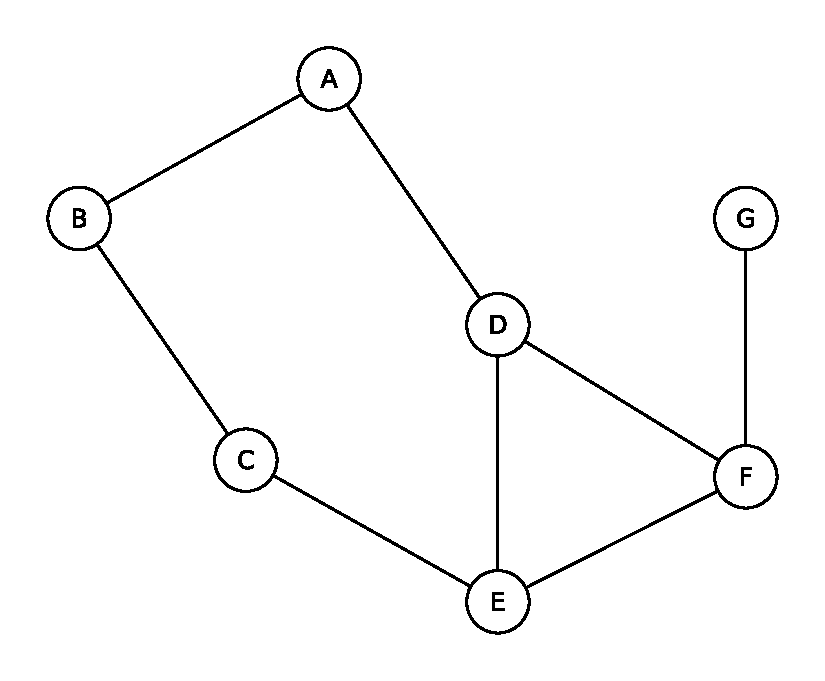
\includegraphics[scale=.55]{../imgs/coeficiente_agrupamento_1.eps}
    }%
    \subfloat[Depois de novas arestas se formarem]{%
      \label{fig:coeficiente_agrupamento_depois}
      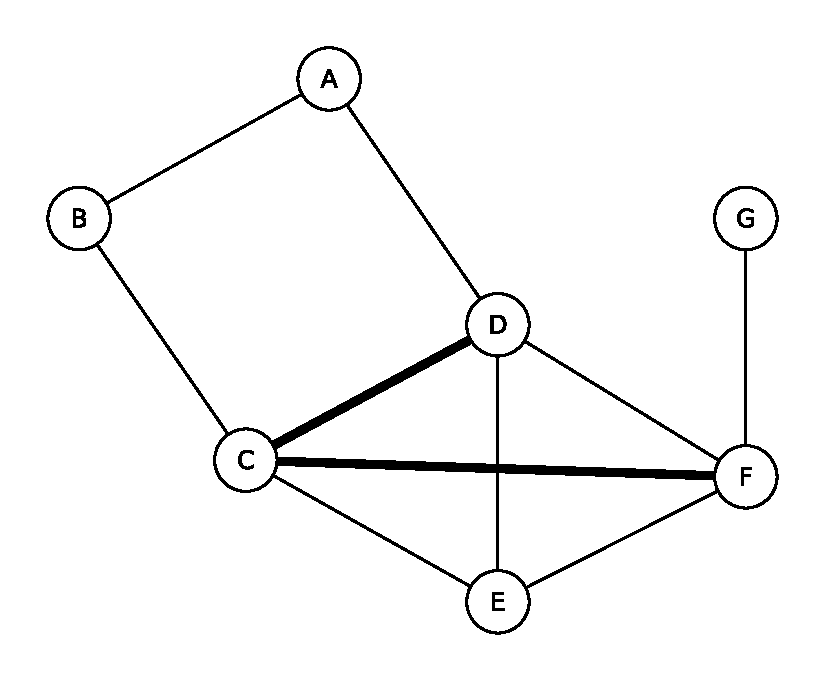
\includegraphics[scale=.55]{../imgs/coeficiente_agrupamento_2.eps}
    }%
  \end{center}
\caption{Exemplo de coeficiente de agrupamento}
\label{fig:averange_values_resemblance}
\end{figure}


%%%%%%%%%%%%%%%%%%%%%%%%%%%%%%%%%%%
\subsection{Componentes}
%%%%%%%%%%%%%%%%%%%%%%%%%%%%%%%%%%%

Segundo \cite{Easley2010}, um grafo é conectado quando existem arestas interligando todos os seus nodos. Naturalmente, 
um grafo é desconectado quando nem todos os seus nodos estão interligados, de modo que eles se dividem em grupos de nodos 
interconectados entre si, porém desconectados do restante da rede, sendo que dois grupos não se sobrepõem. Na 
Figura~\ref{fig:componentes_conectados}, podemos considerar que o grafo consiste de três partes, ou seja, três componentes
conectados: um composto pelos nodos \textit{K}, \textit{I}, \textit{J} e \textit{H}, outro composto pelos nodos 
\textit{L} e \textit{M} e o terceiro composto pelos demais nodos. Por exemplo, em uma rede de coautoria, poderíamos dizer
que cada componente é um grupo de pesquisa, sendo que os pesquisadores de um dado grupo não trabalham com pesquisadores
de outro grupo.

\cite{Easley2010} definem um componente conectado (\textit{connected component}), formalmente, como um subconjunto de 
nodos, tal que: (i) exista um caminho interligando todos os nodos daquele subconjunto e (ii) o subconjunto não é parte 
de um conjunto maior, onde cada nodo possa chegar a qualquer outro. Assim, podemos intuitivamente
definir que um componente é: (i) internamente conectado e (ii) como um todo, é uma ``parte'' 
desconectada das demais partes do grafo. Por exemplo, o subconjunto \textit{C}, \textit{F} e \textit{E} da 
Figura~\ref{fig:componentes_conectados} não poderia ser chamado de componente conectado, pois violaria a 
condição (ii). Embora o subconjunto atenda a condição (i), ele faz parte de um subconjunto maior que engloba 
o nodos de \textit{A} a \textit{G}.

\begin{figure}[!htb]
\centering
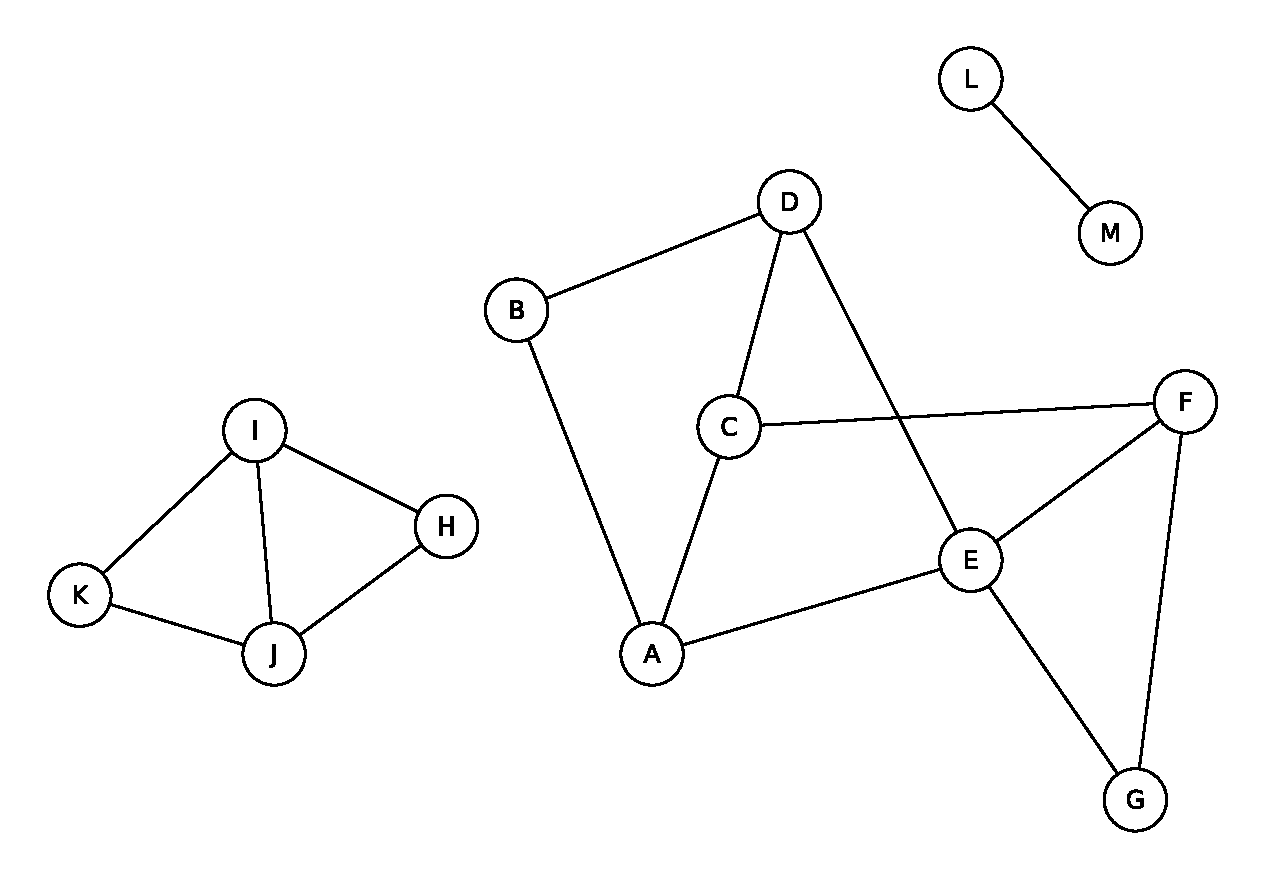
\includegraphics[scale=0.55]{../imgs/componentes.eps}
\caption{Um grafo com três componentes conectados}
\label{fig:componentes_conectados}
\end{figure}

Em um grafo direcionado, um componente é chamado de fortemente conectado quando existe pelo menos um caminho 
direcionado interligando todos os pares de nodos. Quando tal caminho existe, porém não direcionado, o componente 
é chamado de fracamente conectado. \cite{Benevenuto2012} exemplificam o modelo \textit{bow tie}, definido 
por \cite{Broder2000}, em que um grafo possui um componente central fortemente conectado, 
também chamado de \textit{core}, que pode ser alcançado ou alcançar outros grupos de componentes.

%%%%%%%%%%%%%%%%%%%%%%%%%%%%%%%%%%%
% \subsubsection{Maior Componente Conectado?}
%%%%%%%%%%%%%%%%%%%%%%%%%%%%%%%%%%%


%%%%%%%%%%%%%%%%%%%%%%%%%%%%%%%%%%%
\subsection{Caminho Mínimo Médio e Diâmetro}
%%%%%%%%%%%%%%%%%%%%%%%%%%%%%%%%%%%

Os caminhos de uma rede são um aspecto importante dela. Um caminho pode ser definido como uma sequência de nodos sem repetição
onde existe uma aresta entre cada par de nodos adjacentes na sequência. Por exemplo, na Figura~\ref{fig:componentes_conectados}
podemos dizer que existe um caminho entre \textit{A} e \textit{F}, sendo este caminho formado pelas arestas \textit{A-E} e 
\textit{E-F}. O comprimento de um caminho é dado pelo número de arestas que o define ou pelo número de nodos contidos no caminho
menos um. Ainda na Figura~\ref{fig:componentes_conectados}, o caminho contendo os nodos \textit{A}, \textit{B}, \textit{D}, \textit{C} e \textit{F} possui 
tamanho quatro.

Naturalmente existem muitos caminhos entre dois nodos quaisquer de um componente. Desta forma, o caminho mínimo entre
dois nodos é definido como sendo o comprimento do menor caminho entre eles. Assim, considerando os nodos  
\textit{A} e \textit{F} na Figura~\ref{fig:componentes_conectados}, o caminho mínimo entre eles é dois, definida pelos caminhos 
\textit{A}, \textit{C} e \textit{F} ou \textit{A}, \textit{E} e \textit{F}. 

O caminho mínimo médio de um grafo é a média do número de arestas em todos os caminhos mínimos existentes entre todos os pares 
de nodos do grafo. Geralmente esta medida é calculada no maior componente fortemente conectado para grafos direcionados ou no maior 
componente fracamente conectado para grafos não direcionados, uma vez que o grafo pode não ser totalmente conectado. \cite{Figueiredo2011} define 
o caminho mínimo médio como a média aritmética dos caminhos mínimos entre todos os pares de nodos da rede, sendo $l(i,j)$ o caminho mínimo entre os nodos
$i,j \in N$, onde $N$ é o conjuntos de nodos da rede. O caminho mínimo médio $\textit{\=l}$ é definido como:

\begin{equation}
\label{eq:distancia_media}
\textit{\=l} = \frac{\sum_{i,j \in N}{l(i,j)}}{\binom{n}{2}}.
\end{equation}

A Equação~\ref{eq:distancia_media} considera todos os pares não-ordenados, que ao todo são $\binom{n}{2}$. Outra métrica baseada 
em caminho mínimo é o diâmetro que também é calculado no maior componente fortemente conectado ou fracamente conectado. O 
diâmetro é o tamanho do maior caminho mínimo existente em todo o grafo, que \cite{Figueiredo2011} define como:

\begin{equation}
\label{eq:diametro}
\textit{L} = \max_{i,j\in N} l(i,j).
\end{equation}


%%%%%%%%%%%%%%%%%%%%%%%%%%%%%%%%%%%
\subsection{\textit{Betweenness}}
%%%%%%%%%%%%%%%%%%%%%%%%%%%%%%%%%%%

\textit{Betweenness} é uma métrica de centralidade que mede a importância de um determinado nodo ou aresta na rede 
referente à sua localização, considerando o número de caminhos mínimos que por ali passam. Nodos ou arestas com maior 
valor de \textit{betweenness} fazem parte de um número maior de caminhos mínimos e por isto são mais importantes na rede.

O valor da métrica \textit{betweenness} $B(e)$ de uma aresta $e$ pode, de acordo com \cite{Benevenuto2012}, ser formalmente definido como o 
número de caminhos mínimos entre todos os pares de nodos que passam por $e$. Desta forma temos:

\begin{equation}
\label{eq:betweenness}
B(e)=\sum_{u \in N, v \in N} \frac{\sigma_e (u,v)}{\sigma (u,v)}
\end{equation}
onde $\sigma (u,v)$ representa o número de caminhos mínimos entre $u$ e $v$, e $\sigma_e (u,v)$ representa o número de 
caminhos mínimos que incluem $e$. Assim, se existem vários caminhos mínimos entre $u$ e $v$, cada caminho recebe
um peso de modo que o somatório dos pesos seja um.

De forma análoga, o valor da métrica \textit{betweenness} pode ser computado para um nodo da rede ao invés de uma aresta. Assim teríamos
essa métrica representando a importância de um dado nodo para a rede, onde os vários caminhos mínimos que passam
por ele representam, de forma quantitativa, sua importância na rede. Por exemplo, em uma rede de coautoria, a existência de nodos com um alto valor
para a métrica \textit{betweenness} pode indicar que os respectivos pesquisadores atuam como pontes interligando vários grupos de pesquisa na rede. 
Desta forma, adotamos esta métrica de centralidade no restante da dissertação.

%%%%%%%%%%%%%%%%%%%%%%%%%%%%%%%%%%%
\subsection{Assortatividade}
%%%%%%%%%%%%%%%%%%%%%%%%%%%%%%%%%%%

A assortividade (\textit{assortativity} ou \textit{assortative mixing}) é uma métrica clássica de redes complexas que identifica
o comportamento de como os nodos tendem a se agrupar na rede, e.g., uma rede de coautoria apresenta propriedades assortativas 
quando pesquisadores com o mesmo número de conexões tendem a se conectar com outros pesquisadores com o mesmo número de conexões.

A assortatividade pode ser representada visualmente a partir de um gráfico em que cada grau $k$ encontrado em pelo menos um
nodo da rede é representado pelo grau médio $k_{nn}$ dos vizinhos dos nodos de grau $k$. Em grafos direcionados, este gráfico pode
ser construído separadamente para graus de entrada e graus de saída. Segundo \cite{Ahn2007}, esta métrica também pode ser expressa 
numericamente utilizando o coeficiente de correlação de Pearson:

\begin{equation}
\label{eq:assortatividade}
r = \frac{\langle k_ik_j \rangle-\langle k_i \rangle \langle k_j \rangle }
         {\sqrt{(\langle k^2_i \rangle - \langle k_i \rangle^2)(\langle k^2_j \rangle - \langle k_j \rangle^2)}}
\end{equation}
onde $k_i$ e $k_j$ são os graus dos nodos que constituem uma aresta e a notação $\langle \rangle$ representa a média sobre 
todas as arestas da rede.

Se a rede possui assortatividade negativa, nodos que possuem grau elevado tendem a se conectar a nodos com menor grau,
e vice versa. O coeficiente $r$ pode variar entre -1 e 1, onde $r > 0$ indica que a rede possui propriedades assortativas,
ou seja, nodos com graus semelhantes tendem a estabelecer conexões na rede, já $r < 0$ indica que a rede possui
propriedades disassortativas, existindo maior probabilidade de encontrar arestas entre nodos de graus diferentes.
Por exemplo, uma rede de coautoria com assortatividade negativa pode indicar que os pesquisadores seniores estão se
conectando a pesquisadores menos experientes, e.g., alunos de doutorado.

% %%%%%%%%%%%%%%%%%%%%%%%%%%%%%%%%%%%
\section{Modelos de Redes Complexas}
%%%%%%%%%%%%%%%%%%%%%%%%%%%%%%%%%%%

A análise de padrões em redes complexas instigaram vários trabalhos que tiveram como resultados modelos
que descrevem e caracterizam tais padrões. Nesta seção são descritos quatro modelos de redes complexas: 
redes aleatórias, redes \textit{small-world}, redes \textit{power-law} e livres de escala.

%%%%%%%%%%%%%%%%%%%%%%%%%%%%%%%%%%%
\subsection{Redes Aleatórias}
%%%%%%%%%%%%%%%%%%%%%%%%%%%%%%%%%%%

a

%%%%%%%%%%%%%%%%%%%%%%%%%%%%%%%%%%%
\subsection{Redes \textit{Small-World}}
%%%%%%%%%%%%%%%%%%%%%%%%%%%%%%%%%%%

%%%%%%%%%%%%%%%%%%%%%%%%%%%%%%%%%%%
\subsection{Redes \textit{Power-Law} e Livres de Escala}
%%%%%%%%%%%%%%%%%%%%%%%%%%%%%%%%%%%


